In the following, we present the modeling developed for this problem, and
highlight aspects that are relevant for its implementation.

\subsubsection*{Problem}

A problem instance is defined by the set of all libraries available, along with
their sign-up times, book shipping rate, and list of books that can be shipped,
the scores for all the books, and the deadline.

\subsubsection*{Solution}
The solution in this problem is defined by a collection of assignments of books
to libraries and the order in which libraries are scanned. It is important to
note that, in the context of this problem, any partial solution is considered
feasible.

\subsubsection*{Component}

One type of component is a tuple containing a book and library, representing an
assignment. Moreover, given that libraries need to be signed-up in order be
possible to scan books, another type of component is a pair of libraries
$(i, j)$ where, $i = 0, \ldots, \mathcal{L}$ and $j = 1, \ldots, \mathcal{L}$;
denoting that library $j$ is signed-up after library $i$. To denote the first
library that is signed up we consider the component $(0, j)$.


\subsubsection*{Construction Rules}

For this problem, we considered two construction rules which are described as follows:

\paragraph*{Standard}

This approach encompasses enumerating all possible combinations of already
signed-up libraries and not yet scanned books. Additionally, it also enumerates
all libraries that can be signed-up next before the deadline.

\paragraph*{Sequential}

This approach is a slight variation of the previous one. Instead of enumerating
all possible books for all signed-up libraries simultaneously, it only generates
assignments for the last signed-up library and enumerates the books strictly for
that library.~Note that, the selection of which library to sign-up next is also
an enumerated component. As a result, we reduce the complexity of the
enumeration of all components by a factor of~$\mathcal{L}$.

\subsubsection*{Objective Function}

The objective function for this problem is the same as the one defined in the
problem description.

\subsubsection*{Upper Bound}

A possible bound for this problem is to consider each library as a knapsack
problem where the capacity is the number of books that can still be signed-up by
a library until the deadline, and each book represents an item with weight of 1
and profit equal to its score. Note that, for libraries already signed-up the
time until the deadline is known, whereas for libraries that have not yet been
signed up that time is not known. However, we can consider that each not signed
up library will be the next to open, thus relaxing the constraint that dictates
that two libraries can not be signed-up simultaneously. The bound for this
problem is then the sum of a knapsack bound for all libraries considering only
the books that have not yet been signed up and that are available for each
library. Note that, we are also relaxing the fact that each book can only score
once by possibly counting it for the bound of multiple libraries.

Another bound for this problem, is to consider the number of books that can be
shipped until the deadline for all libraries as the knapsack.~Thus, we relax the
constraint set on the number of books that can be scanned for a particular
library imposed by the objective function. Additionally, we consider that a book
can be placed in the knapsack regardless of which library it belongs to. The
association with a specific library is taken into account once the book is
actually scanned. The value of this upper bound is determined by the sum of the
scores of the unique books that can fit within the knapsack.

\subsubsection*{Local Moves}

The local moves considered for this problem include:

\begin{enumerate}
  \item Adding a book to the set of books to be scanned by a given library.
  \item Removing a book from the set of books that were going to be scanned by a
        library.
  \item Swapping books between libraries. This move ensures that both libraries
        have copies of the books being swapped.
  \item Removing a book from the list of books to be scanned by a library and
        adding that book to another library. If possible, replace the removed book in
        the first library with another one that is available there.
\end{enumerate}

\subsubsection*{Perturbation}

Regarding the perturbation of the solution, for this problem, we did not employ
any specific operation apart from randomly applying the described local moves.

\subsection{Two-Phase Approach}

The previous model, although valid, was not competitive in practice. Therefore,
an alternative strategy for modeling this problem was developed. This strategy
involved breaking down the optimization tasks into two distinct stages. The
first stage focused on finding an good order for the libraries, and the second
stage employed an algorithm to assign books to the libraries, effectively
solving the problem.

\subsubsection*{Construction Rules}

The library selection strategy employed was based on a heuristic value
calculated at each step for each library not yet signed-up.~The objective was to
rank the libraries according to their potential contribution given by the books
they contained. There are numerous possible criteria for ranking libraries, such
as prioritizing those with the shortest sign-up time, libraries containing the
rarest books, or libraries with the highest score, among others. However, the
most effective heuristic value for ranking libraries in practice was the one
that takes into account libraries with the highest cumulative score of books not
present in any of the assigned libraries and could be shipped before the
deadline, divided by the sign-up time.

After iteratively selecting libraries based on their heuristic values until it is
no longer possible and defining the library order, we can then solve the book
assignment optimally using an exact method. There are various algorithms in the
literature to solve assignment problems, such as the~\emph{Hungarian
  Method}~\cite{ramshaw2012minimumcost}. However, these algorithms require, in
general, the use of an assignment matrix, which for the instances of this
problem becomes too large and impractical due to memory constraints.

The alternative approach considered involved modeling the problem as a bipartite
graph and using the~\emph{max-flow min-cost} algorithm~\cite{ramshaw2012minimumcost}
to determine the assignment. In this approach, books and libraries were
represented as nodes, and the presence of each book in a library was represented
as an edge. Additionally,~\emph{source} and~\emph{sink} nodes were added to the
graph as required by the algorithm. The bipartite graph is illustrated
in~\Cref{fig:bs-graph}, where there are 3 books and libraries, and book 2 is
present in two libraries simultaneously.

\begin{figure}[h]
  \centering
  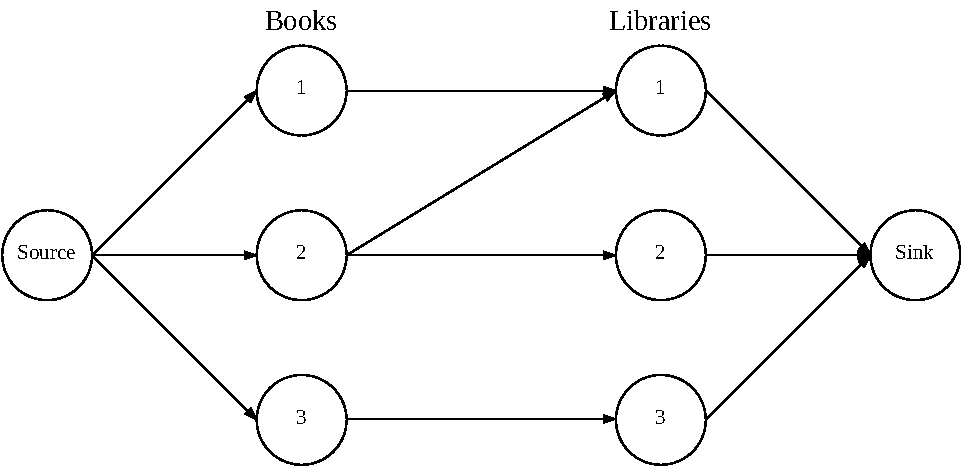
\includegraphics[width=\textwidth,keepaspectratio]{../assets/bs/bs-graph.pdf}
  \caption{Assignment Problem Modeled as a Bipartite Graph}
  \label{fig:bs-graph}
\end{figure}

The edges of the graph are then adjusted in the following way:

\begin{description}
  \item[From \textbf{Source} to \textbf{Books}.] The cost of the edge was set
    to $0$ since we do not wish to count the contribution of this edge, and the capacity
    was set to $1$, symbolizing that all books can be considered for assignment.

  \item[From \textbf{Books} to \textbf{Libraries}.] The cost was set to -$s_{b}$ to
    formulate the problem for maximization, and the capacity was set to $1$, symbolizing
    that each book can be assigned once to that particular library, thereby
    contributing with its score.

  \item[From \textbf{Libraries} to \textbf{Sink}.] The cost was set to $0$
    since libraries do not contribute to the score, and the capacity was given a value
    equal to the number books can be placed in that library, until the deadline~$\mathcal{D}$.
\end{description}

It is important to note that, the assignment will correspond to edges in the
graph that maximize the flow, and secondarily minimize the cost.

\subsubsection*{Local Moves}

To further improve the objective value, we can experiment with different library
orderings by applying the following local moves to the existing order,$\phi^\mathcal{I}$.

\begin{itemize}
  \item Reverse the sign-up order between two libraries in $\phi^\mathcal{I}$
  \item Change the positions of two libraries in the order $\phi^\mathcal{I}$,
        adjusting the sign-up times of every library in between.
  \item Select one library to remove and add another library that is not
        currently considered in that position, if possible.
\end{itemize}